\documentclass{article}
\usepackage{tikz}
\usetikzlibrary{arrows.meta}

\begin{document}

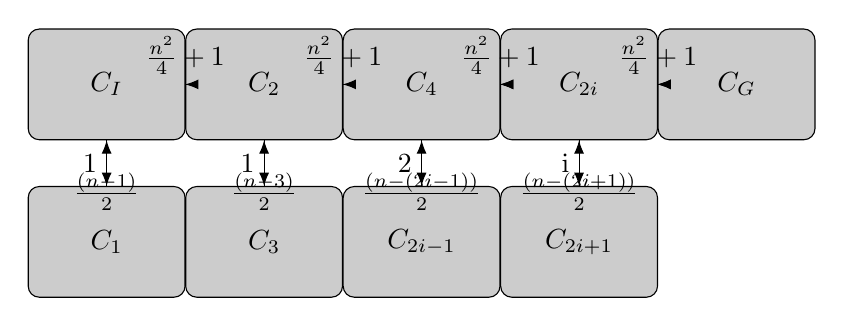
\begin{tikzpicture}[node distance=2cm]
    \tikzstyle{block} = [rectangle, draw, fill=black!20, 
                         text width=5em, text centered, rounded corners, minimum height=4em]
    \tikzstyle{line} = [draw, -Latex]

    % Nodes
    \node [block] (C1) {$C_I$};
    \node [block, right of=C1] (C2) {$C_2$};
    \node [block, right of=C2] (C3) {$C_4$};
    \node [block, right of=C3] (C4) {$C_{2i}$};
    \node [block, right of=C4] (CG) {$C_G$};

    \node [block, below of=C1] (C1b) {$C_1$};
    \node [block, below of=C2] (C2b) {$C_3$};
    \node [block, below of=C3] (C3b) {$C_{2i-1}$};
    \node [block, below of=C4] (C4b) {$C_{2i+1}$};

    % Edges
    \path [line] (C1) -- node [above] {$\frac{n^2}{4} + 1$} (C2);
    \path [line] (C2) -- node [above] {$\frac{n^2}{4} + 1$} (C3);
    \path [line] (C3) -- node [above] {$\frac{n^2}{4} + 1$} (C4);
    \path [line] (C4) -- node [above] {$\frac{n^2}{4} + 1$} (CG);

    \path [line] (C1) -- node [left] {1} (C1b);
    \path [line] (C2) -- node [left] {1} (C2b);
    \path [line] (C3) -- node [left] {2} (C3b);
    \path [line] (C4) -- node [left] {i} (C4b);

    \path [line] (C1b) -- node [below] {$\frac{(n-1)}{2}$} (C1);
    \path [line] (C2b) -- node [below] {$\frac{(n-3)}{2}$} (C2);
    \path [line] (C3b) -- node [below] {$\frac{(n-(2i-1))}{2}$} (C3);
    \path [line] (C4b) -- node [below] {$\frac{(n-(2i+1))}{2}$} (C4);

    \path [dotted, line] (C3) -- (C4);
    \path [dotted, line] (C4) -- (CG);
\end{tikzpicture}

\end{document}